%!TEX program = xelatex
%%%%%%%%%%%%%%%%%%%%%%%%%%%%%%%%%%%%%%%%%
% Short Sectioned Assignment
% LaTeX Template
% Version 1.0 (5/5/12)
%
% This template has been downloaded from:
% http://www.LaTeXTemplates.com
%
% Original author:
% Frits Wenneker (http://www.howtotex.com)
%
% License:
% CC BY-NC-SA 3.0 (http://creativecommons.org/licenses/by-nc-sa/3.0/)
%
%%%%%%%%%%%%%%%%%%%%%%%%%%%%%%%%%%%%%%%%%

%----------------------------------------------------------------------------------------
%	PACKAGES AND OTHER DOCUMENT CONFIGURATIONS
%----------------------------------------------------------------------------------------

\documentclass[paper=a4, fontsize=11pt]{scrartcl} % A4 paper and 11pt font size
\usepackage{xeCJK}
\usepackage[T1]{fontenc} % Use 8-bit encoding that has 256 glyphs
\usepackage{fourier} % Use the Adobe Utopia font for the document - comment this line to return to the LaTeX default
\usepackage[english]{babel} % English language/hyphenation
\usepackage{amsmath,amsfonts,amsthm} % Math packages
\usepackage{amssymb}
\usepackage{lipsum} % Used for inserting dummy 'Lorem ipsum' text into the template
\usepackage{enumerate}
\usepackage{sectsty} % Allows customizing section commands
\usepackage{indentfirst}
\usepackage{hyperref}
\allsectionsfont{\normalfont\scshape} % Make all sections centered, the default font and small caps

\usepackage{fancyhdr} % Custom headers and footers
\pagestyle{fancyplain} % Makes all pages in the document conform to the custom headers and footers
\fancyhead{} % No page header - if you want one, create it in the same way as the footers below
\fancyfoot[L]{} % Empty left footer
\fancyfoot[C]{} % Empty center footer
\fancyfoot[R]{\thepage} % Page numbering for right footer
\renewcommand{\headrulewidth}{0pt} % Remove header underlines
\renewcommand{\footrulewidth}{0pt} % Remove footer underlines
\setlength{\headheight}{13.6pt} % Customize the height of the header

\numberwithin{equation}{section} % Number equations within sections (i.e. 1.1, 1.2, 2.1, 2.2 instead of 1, 2, 3, 4)
\numberwithin{figure}{section} % Number figures within sections (i.e. 1.1, 1.2, 2.1, 2.2 instead of 1, 2, 3, 4)
\numberwithin{table}{section} % Number tables within sections (i.e. 1.1, 1.2, 2.1, 2.2 instead of 1, 2, 3, 4)

\setlength\parindent{2em} % Removes all indentation from paragraphs - comment this line for an assignment with lots of text

%----------------------------------------------------------------------------------------
%	TITLE SECTION
%----------------------------------------------------------------------------------------

\newcommand{\horrule}[1]{\rule{\linewidth}{#1}} % Create horizontal rule command with 1 argument of height

\title{
\normalfont \normalsize
\textsc{Zhiyuan College, Shanghai Jiaotong University} \\ % Your university, school and/or department name(s)
\horrule{0.5pt} \\[0.4cm] % Thin top horizontal rule
\huge CS396: Computational Complexity Homework III \\ % The assignment title
\horrule{2pt} \\ % Thick bottom horizontal rule
}

\author{Zihao Ye} % Your name

\date{\normalsize\today} % Today's date or a custom date

\begin{document}

\maketitle % Print the title

\section*{Exercise 4.10}
Consider the QBF:
$$Q = \exists x_1 \forall x_2 \exists \cdots \forall/\exists x_n \phi(x_1, x_2, \cdots, x_n)$$

\begin{itemize}
	\item $Q = \textit{true}$ implies player 1 has a winning strategy.
	\item $Q = \textit{false}$ implies 
	$$\overline{Q} = \forall x_1 \exists x_2 \forall \cdots \exists/\forall x_n \phi(x_1, x_2, \cdots, x_n) = \textit{true} $$
	Which means player 2 has a winning strategy.
\end{itemize}


\section*{Exercise 4.11}
Suppose $L \in \textrm{coNSPACE}\left(S(n)\right)$, then $\overline{L} \in \textrm{NSPACE}\left(S(n)\right)$, since $S$ is space constructible, by constructing the configuration graph of $L$ on a turing machine, we derive 
$$\forall x, x\in L \iff  \overline{\textrm{PATH}}(G(x), s, t) = 1$$
In which the graph size is $2^{S(|x|)}$. Then according to the fact that $\overline{\textrm{PATH}} \in \textrm{NL}$, we have 
$$ L \in \textrm{NL}\left(2^{S(n)}\right) = \textrm{NSPACE}\left(S(n)\right) $$

For the same reason, we derive $$L \in \textrm{NSPACE}\left(S(n)\right) \Longrightarrow L \in \textrm{coNSPACE}\left(S(n) \right) $$
Combine the results above, $\textrm{NSPACE} = \textrm{coNSPACE}$ will be derived.

\section*{Exercise 5.5}
We first prove that $$\textrm{ATIME}(T(n)) \subseteq \textrm{SPACE}(T(n))$$

For every $L \in \textrm{ATIME}(T(n))$, given an exact input $x$, by traversing the configuration tree(Assume that $T(n)$ is time-constructible) of $M_L(x)$(which requires additional space no more than $O(T(n))$), we could decide whether $x\in L$.

Thus we derive $\textrm{ATIME}(T(n)) \subseteq \textrm{SPACE}(T(n))$, which means $$\textrm{AP} \subseteq \textrm{PSPACE}$$

For the other direction, for every $L \in \textrm{SPACE}(P(n))$, given an input $x$ with length $n$, considering the {\bf Divide and Conquer} method we used in proving {\it Savitch Theorem}.

The configuration graph has $M = 2^{P(n)}$ nodes. We need to construct an ATM to decide whether $C_{accept}$ is reachable from $C_{start}$.

The {\bf Divide and Conquer} algorithm could be described as:

\begin{figure}[!htb]
\centering
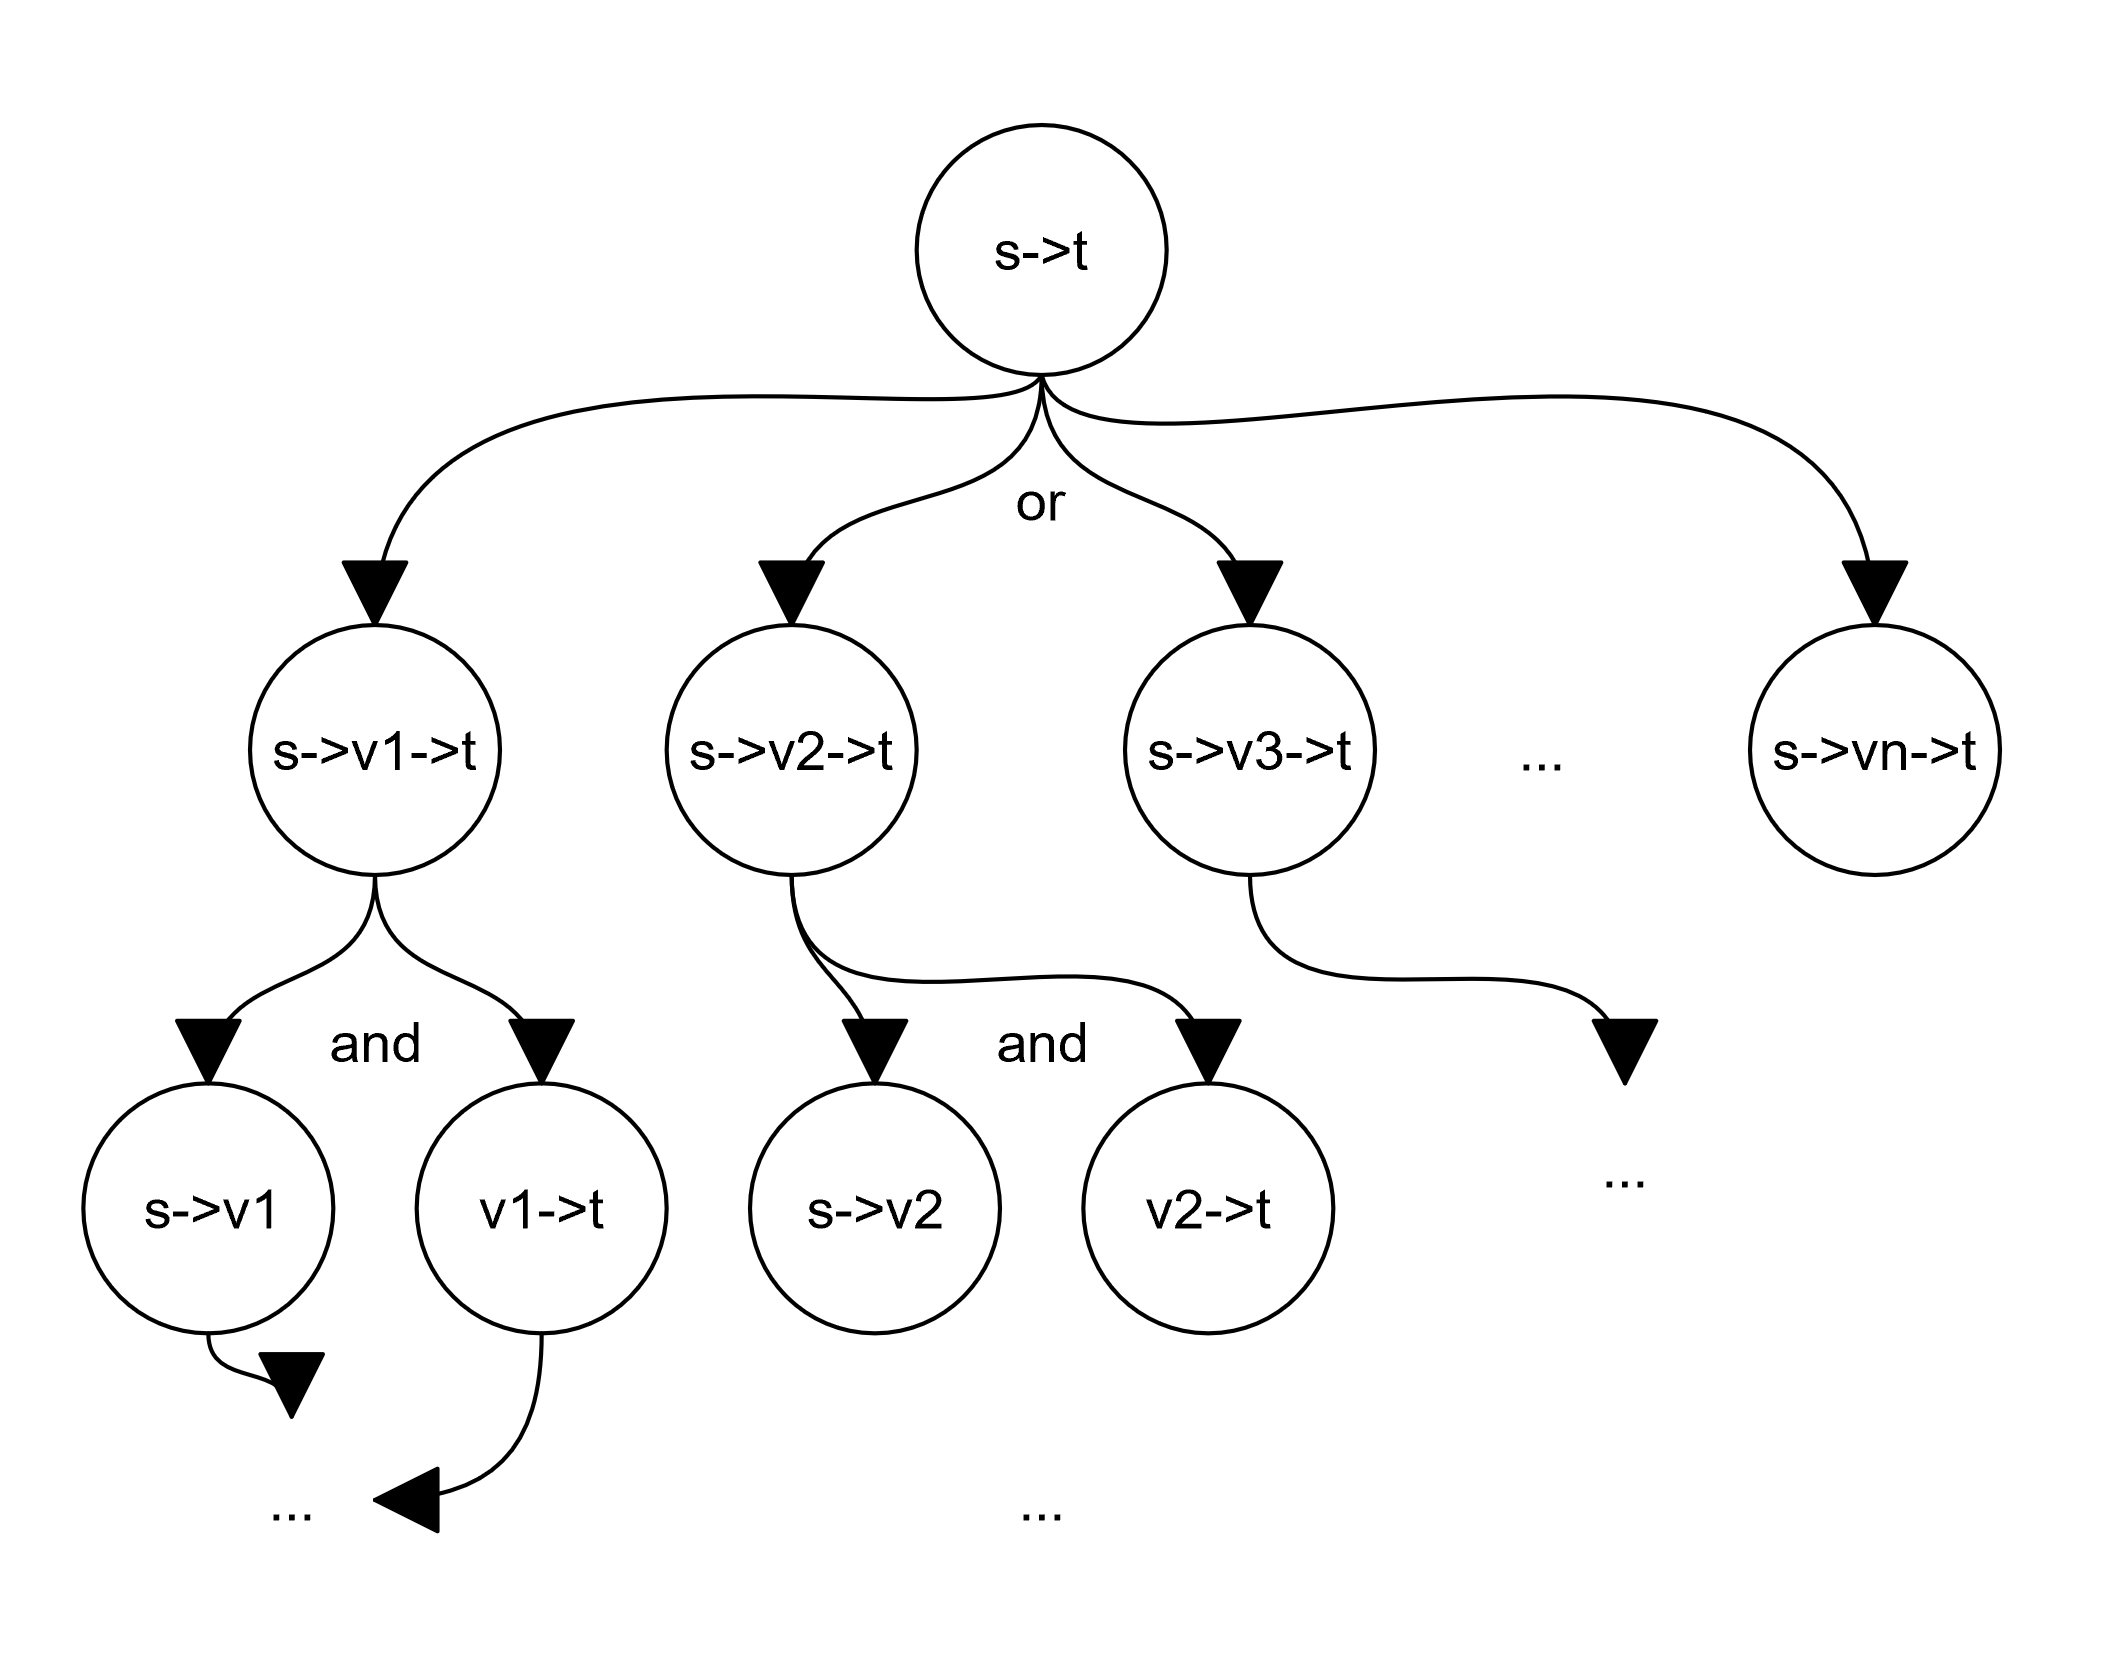
\includegraphics[width=300pt]{savitch.png}
\end{figure}

Multiple branch($k$ of them at all) could be converted to $log(k)$ layers of binary branch structures.

Thus the tree's depth is no more than $O(log^2(M)) = P(n)^2$. We could decide whether $x\in L$ in $\textrm{ATIME}(P(n)^2) \subseteq \textrm{AP}$.

Combine the results above, we have $$\textrm{AP} = \textrm{PSPACE} $$

\section*{Exercise 5.9}
\subsection*{I}
$$(G, k) \in \textrm{EXACT INDSET} \iff \forall S\subseteq V, \exists S'\in V, \left(S' \in \textrm{INDSET}, |S'| = k, S' \subseteq S \Longrightarrow S \not\in \textrm{INDSET}\right)$$
\subsection*{II}
$$(G, k) \in \textrm{EXACT INDSET} \iff (G, k) \in \textrm{INDSET} \wedge (G, k + 1) \not\in \textrm{INDSET} $$

While $\textrm{INDSET} \in \textrm{NP}$, $\{(G, k)\mid (G, k) \not \in \textrm{INDSET}\} \in \textrm{coNP}$, thus:
$$(G, k) \in \textrm{DP} $$ 
\subsection*{III}

For each $L \in \textrm{DP}$, Suppose $L = L_1 \cap L_2$, while $L_1\in\textrm{NP}$ and $L_2\in\textrm{coNP}$.

We could make a reduction from $L\in \textrm{NP}$ to a $3\textrm{SAT}:\phi$, furthermore an $\textrm{INDSET}:(G,k)$. While a $L \in \textrm{coNP}$ could be reduced to an $\overline{\textrm{INDSET}}$ problem. Suppose these two reductions are $\phi_1 \rightarrow (G_1, k_1)$ and $\phi_2 \rightarrow (G_2, k_2)$, respectively.

Such reduction doesn't not suggest any lower bound for largest size of independent set. So we introduce $k_i-1$ new nodes for each reduction, and add edges from new nodes to all existing nodes. However this augmentation guarantee that largest size of independent size can't be lower than $k_i - 1$.

Construct a new graph $G_1\times G_2$ as described below:
$$V = V_1 \times V_2$$
$$(\langle v_1, v_2 \rangle, \langle v_1', v_2' \rangle) \in E \iff (v_1, v_1') \in E_1 \vee (v_2, v_2') \in E_2 $$ 

While this construction indicates a indset with size $|\textrm{IND}_1|\cdot |\textrm{IND}_2|$, and in this case, $|\textrm{IND}_1| = k_1, |\textrm{IND}_2| = k_2 - 1$. If $k_1 = k_2$, none of the cases could yield a $\textrm{EXACT\_INDSET}$ with size $k_1(k_2-1)$.

After all these conversions, we could decide whether $x\in L$ by $$\textrm{EXACT\_INDSET}(G, k_1(k_2-1))$$

\section*{Exercise 6.3}

Suppose $B$ is the set used in the proof of {\it Baker-Gill-Solovay Theorem} that satisfies $U_B\in \textrm{NP}^B$ and $U_B\not\in P^B$, in which $U_B = \{1^n \mid \exists b\in B, |b| = n\}$.

While in {\bf Exercise 3.3}, it has been proved $B$ could be made exponentially polynomial decidable.

$P \subseteq P^B$, thus $U_B \not\in P$. While as it's a unary function, according to {\bf Clamin 6.8}, $U_B \in P_{/poly}$.
\section*{Exercise 6.16}

Suppose $A$ is a $n\times n$ matrix. 

Suppose $\lambda_1, \lambda_2, \cdots, \lambda_n$ are $n$ eigenvalues of $A$, $$\det(A) = \prod_{i=1}^{n} \lambda_i$$
In order to compute $\det(A)$ in a circuit with $O(log(n))$ layers, we introduce intermediate variables $\{P_i\}$, $\{E_i\}$ defined as follows:
$$P_i = \sum_{k=1}^{n} \lambda_k^i$$
$$E_i = \sum_{k_1, k_2, \cdots,k_i \in {[n] \choose i}} \lambda_{k_1} \lambda_{k_2} \cdots \lambda_{k_i} $$

For convenience, let $E_0$ be $1$.

Their relations could be formulated as({\it Newton's Identity}):
$$E_i = 1/i \cdot (-1)^{i+1} \sum_{k=1}^{i} P_k E_{i - k}$$

{\it Vieta's formulas} implies $\{(-1)^{i} E_i\}$ are the coefficients of the polynomial $\det(\lambda I - A)$, let $c_i$ be $(-1)^{i} E_i$, then $(-1)^{n}c_n = E_n = \det(A)$.

While we could find the relation between $c_i$ and $P_i$
$$-c_i = 1/i \sum_{k=1}^{i} (-1)^{i - k}P_k c_{i-k}$$

To vectorize this formula, we have to transform it to:
$$-\frac{P_i}{i} = \sum_{k=1}^{i} (-1)^{k - 1}\frac{P_{i - k}}{i} 	c_{k}$$

Whose matrix form is:

$$
\begin{bmatrix} 
-P_1 \\
-\frac{P_2}{2} \\
-\frac{P_3}{3} \\ 
\vdots \\
-\frac{P_n}{n} 
\end{bmatrix} = 
\begin{bmatrix}
1 & 0 & 0 & \cdots & 0 \\
-\frac{P_1}{2} & 1 & 0 & \cdots & 0 \\
-\frac{P_2}{3} & -\frac{P_1}{3} & 1 & \cdots & 0 \\
\vdots & \vdots & \vdots & \vdots & \vdots \\
-\frac{P_{n-1}}{n} & -\frac{P_{n-2}}{n} & -\frac{P_{n-3}}{n} & \cdots & 1 
\end{bmatrix}
\begin{bmatrix}
c_1 \\
c_2 \\
c_3 \\
\vdots \\
c_n
\end{bmatrix}
$$

Use $W$ to denote the weight matrix, then $P = WC$, $C = W^{-1}P$.
Suppose $W = I - L$ ($L$ is a lower-triangular matrix with all-zero diagonal elements), $W^{-1} = I + L + L^2 + \cdots + L^{n-1}$.

To show $$\{\langle M, k\rangle \mid \det(M) = k\} $$ is actually in $NC$, we construct a circuit with $O(\log(n))$ layers and $O(Poly(n))$ gates as follows:

\begin{itemize}
	\item {\bf Addition, Subtraction, Mutliplication and Division Module}: 
	These could be implemented by combining some `AND' and `OR' gates, the number of gates is $O(n)$.
	\item {\bf Sum Module}: 
	Summation of $\{a_i\}$ could be reformulated as:
	$$\sum_{i=1}^n a_i = \sum_{i=1}^{n/2} a_i + \sum_{i = n/2+1}^{n} a_i $$
	Apply the same technique on the first half and the second half, then we derive a module with $O(\log(n))$ layers and $O(n)$ gates.
	\item {\bf Matrix Multiplication Module}:
	Create $n^3$ modules to parallelly compute $A_{ik}B_{kj}$($n^3$ of them). Then use $n^2$ {\bf Sum Module} to parallely compute $AB$. This module has $O(\log(n))$ layers and $O(n^3)$ gates. 
	\item {\bf Matrix Power Module}:
	Use the same technique we used in {\bf Sum Module}, and this could be handled with $O\left(\log^2(n)\right)$ layers and $O(n^4)$ gates.
\end{itemize}

By combining these modules we could construct a circuit to effectively calculate $\det(M)$ with $O\left(\log^c(n)\right)$ layer and $O(Poly(n))$ gates. Thus $\{\langle M, k\rangle \mid \det(M) = k\} \in \textrm{NC}$.

\section*{Acknowledgement}
Thanks Yurong You for his discussion with me.

Thanks Lequn Chen for his generous help on searching some excellent solutions online.

\section*{Reference}
\begin{enumerate}
	\item \url{http://drona.csa.iisc.ernet.in/~chandan/courses/arithmetic_circuits/notes/lec6.pdf}
	\item \url{http://zoo.cs.yale.edu/classes/cs468/spr15/solutions/HW3-Solutions.pdf}
\end{enumerate}
\end{document}

